\documentclass[runningheads]{llncs}

%---- Sonderzeichen-------%
\usepackage[english]{babel}
%---- Codierung----%
\usepackage[latin1]{inputenc}	% for Unix and Windows
\usepackage[T1]{fontenc}
\usepackage{graphicx}
\usepackage{url}
\usepackage{llncsdoc}
%----- Mathematischer Zeichenvorrat---%
\usepackage{amsmath}
\usepackage{amssymb}
\usepackage{enumerate}
% fuer die aktuelle Zeit
\usepackage{scrtime}
\usepackage{listings}
\usepackage{subfigure}
\usepackage{hyperref}
\usepackage{float}

\newcommand{\nocontentsline}[3]{}
\newcommand{\tocless}[2]{\bgroup\let\addcontentsline=\nocontentsline#1{#2}\egroup}

\setcounter{tocdepth}{3}
\setcounter{secnumdepth}{3}

\title{The CoCoME Platform for Collaborative Empirical Research on Information System Evolution}
\author{}%TODO anpassen
\institute{Institute for Program Structures and Data Organization}

\begin{document}
\tocless\maketitle	
	
\tableofcontents

\section{Introduction}

\section{CoCoME Plattform Overview}

\section{Evolution Subject}
In this paper, we use CoCoME as evolution subject. CoCoME has been further evolved in various projects, using the existing Hybrid Cloud-based Variant and a new approach called Microservice-based Variant. The former is sufficiently presented in the official Technical Report of CoCoME. See \cite{SWB-469002735} for any information and implementation details.
\subsection{Hybrid Cloud-based Variant}
The hybrid cloud-based variant of CoCoME was developed in the DFG Priority Programme
Design For Future - Managed Software Evolution (SPP 1593) \cite{Goltz2015}. This variant of CoCoME is using Java EE technologies for both the frontend and the backend. The hybrid cloud-based variant used in this report is completely identical to the variant described in \cite{SWB-469002735}. 

\subsection{Microservice-based Variant}
%TODO Hier muss jetzt eine Übersicht rein, sobald MS fertig implementiert. Dies wird ähnlich zu Technical report sein!
vgl zu 2016,2 Since.. various research projects ggf aendern?
mit 3.1, 3.2, 3.3 gemeint ->?
\chapter{Evolution Scenarios}
We implemented distinct evolution scenarios covering the categories adaptive and perfective
evolution. Corrective evolution is not considered in the scenarios as this merely refers to fixing design or implementation issues.

\section{Evolution Scenarios of the Hybrid Cloud-based Variant}
This section introduces the two evolution scenarios of the hybrid cloud-based variant of
CoCoME.
\subsection{Setting up a Docker environment}
~\\The CoCoME company must reduce IT administration costs but frequent updates to the enterprise and store software are necessary to continuously improve the entire system. As a consequence, IT staff need to update the system components as soon as a new software version is released. An Operations Team member has to get access to the actual server in order to undeploy the old version and replace it with the new one. This is time consuming and expensive as the updates have to be done manually.\\
Therefore, a Docker version is elaborated to simplify the administration process. As soon as a new software version of CoCoME is ready for delivery, the Development Team wrap it into a Docker Image. This Image can be automatically deployed to the destination server according to the principle of Continuous Deployment (CD) \cite{olsson2012climbing}. 




\subsection{Adding a Mobile App}
~\\After successfully adding a Pick-up Shop, the CoCoME company stays competitive with other online shop vendors (such as Amazon). In times of smartphones, customer do not only want to buy exclusively goods from their home computers. Purchasing goods 'on the way' comes more and more into fashion. This raises the idea to create a second sales channel next to the existing Pick-up Shop in the CoCoME system. As a consequence, more customers can be attracted to gain a larger share of the market. 
\\
The customer can order and pay by using the app. The delivery process is similar to the Pick-up Shop: The goods are delivered to a pick-up place (i.e. a store) of her/his choice, for example in the neighbourhood or the way to work.
By introducing the Mobile App as a multi OS application, the CoCoME system has to face various quality issues such as privacy, security and reliability. Also the performance of the whole application can be affected if many customers order via the app.




%TD\newpage

\section{Evolution Scenarios of the Microservice-based Variant}
This section introduces the evolution scenario of the Microservice-based variant of
CoCoME.
\subsection{Defining different Microservices}
After a year of economical stagnation, the CoCoME company decided to restructure its infrastructure. Global players like Amazon or Netflix demonstrated that using a Microservice Architecture makes them more flexible regarding new functionality. When adding the Pick-up Shop, the CoCoME company realized that they have to break open the existing system. It was necessary to modify the \textit{WebService::Inventory} and the \textit{TradingSystem::Inventory} component \cite{SWB-469002735}. Furthermore, adding a \textit{MobileAppClient} demonstrated that the SOAP/WS*-based web services provided by CoCoME are not compatible with REST-based App development.
\\
Inspired by the flexibility and reusability of Microservices, the CoCoME company decided to invest money into a restructuring process. The current system is divided into a collection of loosely coupled services. Each of them cover a specific part of the former CoCoME system. The aim is to preserve the functionality of the current system and solely change its architecture.
\\
 This enables the company to develop new markets much easier and therefore secures the future competitiveness. For example, the CoCoME company wants to extend their product range by offering movie streaming. This requires a vastly different system. Nevertheless, Customer Management like login and means of payment are identical to the former CoCoME system. Those components already exists as a Microservice a therefore can be taken over. The management is certain that this will soon result in economical growth.








	
	

\chapter{Design Details for Evolution Scenarios}
%TODO "describes the adaptive evolution scenari of.." changed to "changes in "
In this chapter we provide the detailed design documentation for each of the evolution scenarios
introduced in the prior section. Sec. \ref{App} sketches the design decision for the Mobile App that provides a second sales channel next to the existing Pick-up Shop. Sec. \ref{Docker} describes the adaptive cahnges of setting up a Docker environment to simplify the update process. They are both based on, or at least use the Hybrid Cloud-based Variant of CoCoME \cite{SWB-469002735}. In contrast, Sec. \ref{MS} provides a detailed design documentation of a new architectural version of CoCoME. This perfective evolution scenario is realized based on the Microservice idea.

\section{Design Decisions for the Mobile App} \label{App}
	%TODO Add most important information od App-Paper	
		\begin{figure}[H]
			\centering
			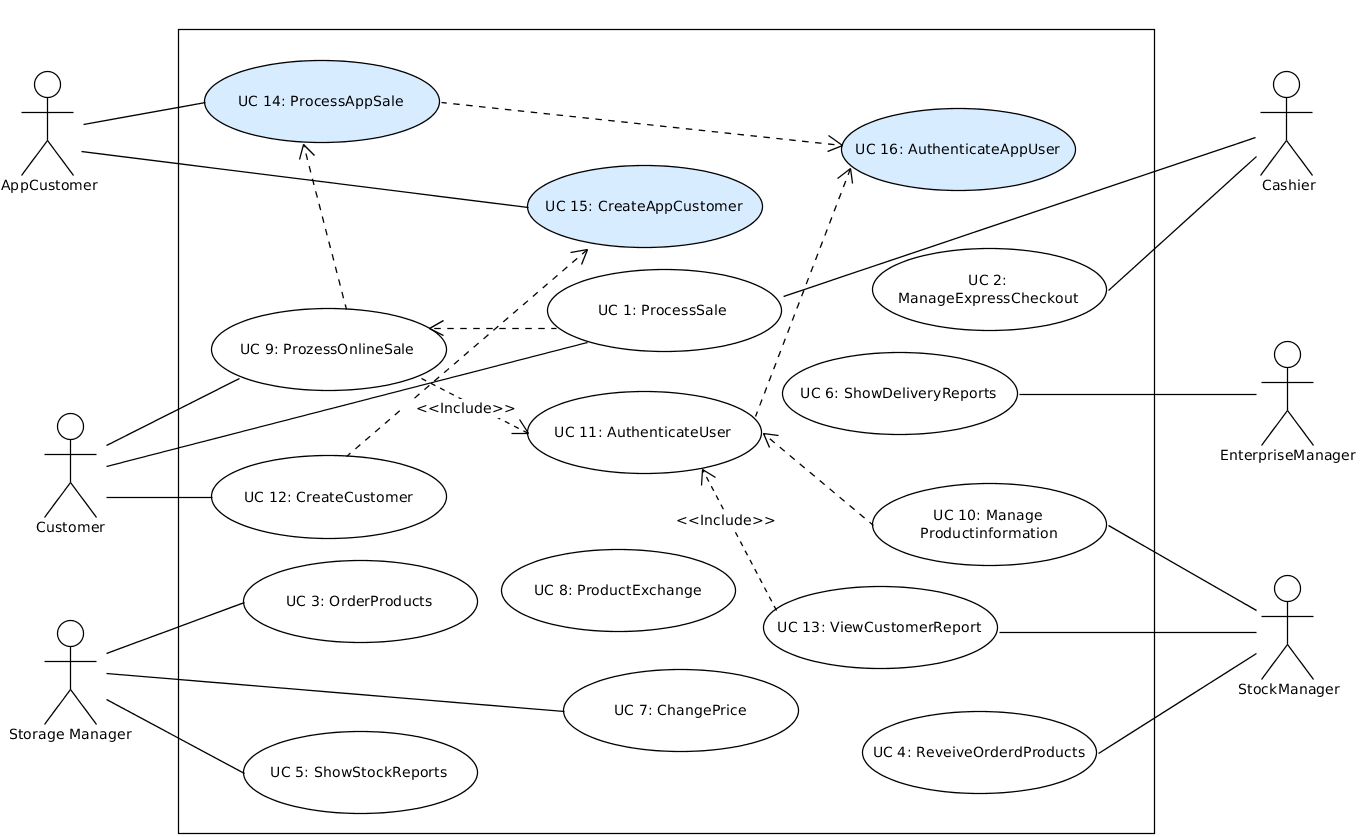
\includegraphics[width= \textwidth]{img/UseCaseApp.png}
			\caption{Use Case Diagram CoCoME Mobile App}
		\end{figure}

\section{Setting up a Docker environment} \label{Docker}
	%TODO Add most important information of docker paper
	Looking to the changes for the Docker project, you can see in figure \ref*{techStack} the changes are affecting the technology stack in the form of adding additional layers. More detailed, the given CoCoME project is moved into the Docker Deamon, which runs a Linux distribution.The original parts of the stack, like Glassfish and the Java Virtual Machine, are still a part of the stack.\\
	\begin{figure}[H]
		\centering
		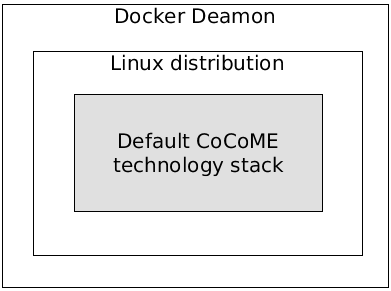
\includegraphics[width = 0.5\textwidth]{img/tech_stack_CoCoME.png}
		\caption{Extended technology stack CoCoME}
		\label{techStack}
	\end{figure}
	
	%TODO important here?
	The Dockerfile defines an environment based on the latest version of Ubuntu 16:04. Onto it there is installed Maven, Git and Java by using the Ubuntu package manager.\\
	Git has two purposes: On the one hand it is used to download the most recent version of CoCoME.	On the other hand, it is used to download a prefabricated version of Glassfish that already includes domains and other adjustments required for CoCoME. Java is required by Glassfish and CoCoME as they need the Java Virtual Machine. Maven is needed to deploy the latest version of CoCoME onto the provided Glassfish servers.
	
	
	During the development, it was decided to implement and provide two different versions. The first version always pulls the most recent CoCoME source code from GitHub, downloads the entire dependencies with maven, compiles and builds the project and finally, deploys CoCoME on the Glassfish servers. . As a consequence. creating and starting a Docker Container takes about one hour.\\
	In contrast, the second version only  pulls a prefabricated version of CoCoME from GitHub. Therefore, pulling the source code up to building the project is skipped. As a consequence, Maven does not have to be included in the technology stack. Solely, deploying CoCoME on the glassfish server is necessary.\\
	This reduces the deployment time to a few minutes but has a disadvantage: The prefabricated version is updated manually. Therefore, it is sometime not the most recent version.\\
	By providing both, a fast deploying version and a current version, the user can choose whats the best for its situation.
	

	

	
\section{Using Microservices Technology} \label{MS}
	\begin{itemize}
		\item je microservice absatz mit entsprechenden Sequenzendiagram %fertig machen der implementierung
		\item frontend? muss dazu auch das gemacht werden?
		\item ein blocktext zu mehereren diagrammen oder diagramme zwischen text?
		
	
			\item je die einzelnen module und szenarien erlaeutern in dem diese sinnvoll sind
	\end{itemize}
	
		\subsection{Products}
		abstrahieren der Produktinformationen 
		
		\subsection{Stores}
		einzelne Laeden alleinstehend abbilden um nach bedarf neue microservices alias laeden starten zu können
		
		\subsection{Enterprise}
		aehnlich zu stroes
		
		\subsection{Reports}
		stellt alleinigen aufgaben bereich dar, entsprechen undabhaengig darzustellen von anderem.


\section{Life-Cycle}
was genau ist hiermit gemeint
\chapter{Implementation of Evolution Scenarios}
gemeint die abh. zwischen den einzelnen klassen?
 - bei mobile app angegeben, alt. wo ist der quellcode?\\
 - docker den techstack (nocheinmal?) angeben?
 - microservices hierzu komplett fertig? oder nur die einzelnen mittelstücke? ohne entsprechende anbindung an frontend/backend?
\section{Conclusion}

\end{document}
